\documentclass[review]{elsarticle}
\usepackage{adjustbox}
\usepackage{tabularx}
\newcommand\setrow[1]{\gdef\rowmac{#1}#1\ignorespaces}
\newcommand\clearrow{\global\let\rowmac\relax}
\clearrow
\usepackage{float}
\usepackage{multirow}
\usepackage{lineno,hyperref}
\usepackage{amsmath}
\usepackage{url}
\usepackage{natbib}
%\modulolinenumbers[5]
\usepackage{lscape}
\usepackage{lineno}
%\linenumbers
\usepackage{subcaption}
%\usepackage{graphicx}
\journal{}

\newcommand{\poubelle}[1]{}
%%%%%%%%%%%%%%%%%%%%%%%
%% Elsevier bibliography styles
%%%%%%%%%%%%%%%%%%%%%%%
%% To change the style, put a % in front of the second line of the current style and
%% remove the % from the second line of the style you would like to use.
%%%%%%%%%%%%%%%%%%%%%%%%%%%%%%%%%%%%%%%%%%%%%%%%%%%%%%%%%%%%%%%%%%%%%%%%%%%%%%%%%%%%

%% Numbered
%\bibliographystyle{model1-num-names}

%% Numbered without titles
%\bibliographystyle{model1a-num-names}

%% Harvard
%\bibliographystyle{model2-names.bst}\biboptions{authoryear}

%% Vancouver numbered
%\usepackage{numcompress}\bibliographystyle{model3-num-names}

%% Vancouver name/year
%\usepackage{numcompress}\bibliographystyle{model4-names}\biboptions{authoryear}

%% APA style
%\bibliographystyle{model5-names}\biboptions{authoryear}

%% AMA style
%\usepackage{numcompress}\bibliographystyle{model6-num-names}

%% `Elsevier LaTeX' style
\bibliographystyle{elsarticle-num}
%%%%%%%%%%%%%%%%%%%%%%%

\begin{document}

\begin{frontmatter}

\title{Parallel Genetic Algorithm for Solving the Graph Partitioning Problem }

%\fntext[myfootnote]{Since 1880.}

%% or include affiliations in footnotes:
\author[mymainaddress,mysecondaryaddress,institutionAdresse]{Ali Chaouche}
\ead{chaouche007@gmail.com}

\author[mysecondaryaddress,institutionAdresse]{Menouar Boulif \corref{mycorrespondingauthor}}
\ead{boumen7@gmail.com}
\cortext[mycorrespondingauthor]{Menouar Boulif}



\address[mymainaddress]{LIMOSE Laboratory}
\address[mysecondaryaddress]{Departement of computer science}
\address[institutionAdresse]{University of M’hamed Bougara of Boumerdes, Facutly of Sciences. Avenue de l'indépendance, 35000. Boumerdes, Algeria}

\begin{abstract}
The performances of genetic algorithms relies heavily on various parameters, particularly the encoding scheme used to represent solutions. This paper introduces a novel parallel genetic algorithm that employs two sub-populations each with a specific encoding scheme. Knowing that each encoding scheme possesses its owns features that may help it to better explore the search landscape or even prevent it to get through promising search areas. This approach aims to mitigate the limitations associated with these encodings and enhance the performance of the genetic algorithm for addressing the graph partitioning problem (GPP) in order to improve enhance the efficacy of the genetic algorithm. The encoding schemes employed in this study include an integer vertex based encoding and a binary edge based encoding. The core concept is the migration of best solutions among the sub-population following a specific strategy. 
\end{abstract}

\begin{keyword}
	 \text k-way graph partitioning problem\sep parallel genetic algorithm\sep encodings schemes\sep solutions migration\sep unsupervised graph partitioning. 
\end{keyword}

\end{frontmatter}
\section{Introduction} 
Since their appearance in 1975s by J.Holland \cite{holland_1975}, genetic algorithm (GAs) still achieve impressive improvement. This stochastic bio-inspired methods are known by their simplicity and effectiveness to solve hard problems. Their principle is rather simple. Indeed, the process consists of evolving iteratively a population of candidates’ solutions throughout a specific process till the fulfillment of a certain condition. Genetic operators such as natural selection, crossover and mutation are applied during the whole process \cite{goldberg1988genetic}.
As a blind method, GAs are strongly relay on their encoding scheme used to represent solutions to better explore the search landscape related to the treated problem \cite{rothlauf_goldberg_2003}.  In their paper \cite{chaouche2019solving} Ali et Menouar had presented a set of encoding schemes used by GAs to solve the graph partitioning problem. However, each of the presented encoding scheme has its limitations and drawbacks. 
The main idea behind this work is to use a parallel GA, in which we make a set of sub-population each with a specific encoding scheme evolve together in order to get advantage of each of these encoding schemes. A migration strategy is applied to get better solutions transferred from a sub-population to anther with the aim of getting the search process of the later redirected to new promising areas \cite{alba1999survey}.
The next of this paper is structured as follow :
In section 1 we provide a description of the graph partitioning problem. Section 2 will be dedicated to the parallel genetic algorithm and the different encoding schemes used by each sub-population. Afterwards, we will thoroughly present our experimental study, and we finish by drawing a conclusion and highlighting some future directions.

\section{Problem Description}
The graph partitioning is widely used in many areas such as community detection in social networks \cite{que2015scalable}, power networks \cite{li2010controlled}, image processing \cite{mittal2022comprehensive}, to cite only few.
In this work we treat the k-way graph partitioning problem. A formal definition of GPP is given as follow :
 given an undirected weighted graph $G=(V,E)$ where $V={v_1,\ldots,v_n}$ is the set of the vertices and $E={e_1, \ldots ,e_m }\subset(V \times V)$ the set of the edges to each we associate a non-negative weights denoted $omega(e)$. The graph partitioning problem asks for a partition $P = {C_1,\ldots,C_k}$ of  $V$ in $k$ blocks of nodes namely clusters that satisfy the following constraints:

\begin{equation}
\forall i,j \in \{1,2,\ldots,k\},i\neq j : C_i\cap C_j= \emptyset
\end{equation}
\begin{equation}
\cup_{i=1}^k  C_i = V
\end{equation}
\begin{equation}
\forall i\in \{1,2,\ldots,k\} : C_i  \neq \emptyset
\end{equation}                                          

\noindent In addition, feasible solution must satisfy the following constraints in order to be accepted:

\begin{itemize}

	
	\item 	Cohabitation  constraints: let $C$ the set of vertex pair that must be in the same cluster.  Coexistence constraints is formulated as follow :
	
	\begin{equation}
	\begin{split}
	\forall (v_k,v_l )\in X, \ k, \ l \in \{1,2,\ldots,|V|\}, \  \exists C_i  \in P, \ i\in \{1,\ldots,|P|\}: \\
	\  v_k, \ v_l\in C_i   	
	\end{split}
	\end{equation}
	
	\item Non Cohabitation  constraints: let $T$ the set of vertex pair that must be in the same cluster. Non coexistence constraints is formulated as follow : 
	
	\begin{equation}
	\begin{split}
	\forall(v_k,v_l )\in Y, \ k, \ l\in \{1,2,\ldots,n\}, \ \exists \ C_i,\ C_j  \in P,
	i,j\in \\ \{1,\ldots,|P|\},  i\neq j : \ v_k \in C_i  \ and \  v_l \in C_j	         
	\end{split}
	\end{equation}
	
	\item Cluster size constraint: the partition's clusters size must be lower than or equal a maximum predefined number of vertices denoted $N$, that is :
	
	\begin{equation}
	\forall i\in \{1,2,\ldots,|P| \}: |C_i |\leq N                                                                            
	\end{equation}
	
\end{itemize} 
% 
The aim of the objective function of the k-way graph partitioning problem is to search for a partition $P^*$ that minimize the sum of the edge cut weight $E_c\subset $defined as follows:

\begin{equation}
E_P = \{  (v_i,v_j ) / (v_i,v_j ) \in E \ and  \ \exists \ C_k,C_l, \ k \neq l  \ : \  v_i  \in C_k \  and \ v_j  \in C_l \}
\end{equation}
\noindent That si:    $\sum_{e\in E_P} \omega(e)$  is minimal.

\section{Parallel Genetic Algorithm (pGA)}
As a matter of clarification, we provide in table \ref{tab:AG} a short description of the genetic process. The main concept behind this method is to mimic the evolution process in which a population of candidates solution undergo iteratively a set of genetic operators.

\begin{table}[H]
	\center
	\label{tab:AG} % pour les référence croisées
	\begin{tabular}{l l l}
		\hline
		& \bf  Algorithm 1 : Genetic Algorithm & \\
		\hline 
		& $t \leftarrow 0$ & \\
		& initialize$(P(t))$ & \\
		& evalute$(P(t))$ & \\
		& \textbf{loop} & \\
		&  \ \ \ \ \ \ \   $t \leftarrow t+1$  &  \\
		&  \ \ \ \ \ \ \  select $P(t+1)$ from $P(t)$ &  \\
		& \ \ \ \ \ \ \   alter$(P(t+1))$ & \\
		& \ \ \ \ \ \ \   evaluate$(P(t+1))$ & \\
		& \textbf{Until(}termination-condition\textbf{)} & \\
		\hline
	\end{tabular}
\end{table}

Traditional genetic algorithms (GAs) suffer from the fact that they use only one encoding scheme to represent solutions. An encoding scheme possesses some characteristics such as blindness which is the incapability of the encoding to represent some kind of solutions in the search space, or redundancy where a single solution may have more than one representation at a time, to name just a few \cite{rothlauf_goldberg_2003}. These intrinsics features may have dramatic consequences on the performances of the GA. 
To overcome these limitations, we propose a parallel genetic algorithm with two distinct sub-populations each of them uses a different encoding. A migration strategy is used to share best solutions of both sub-populations in order to redirect their respective search process to hopefully new promising areas.
\begin{center}
	\begin{figure}[H]
		\centering
		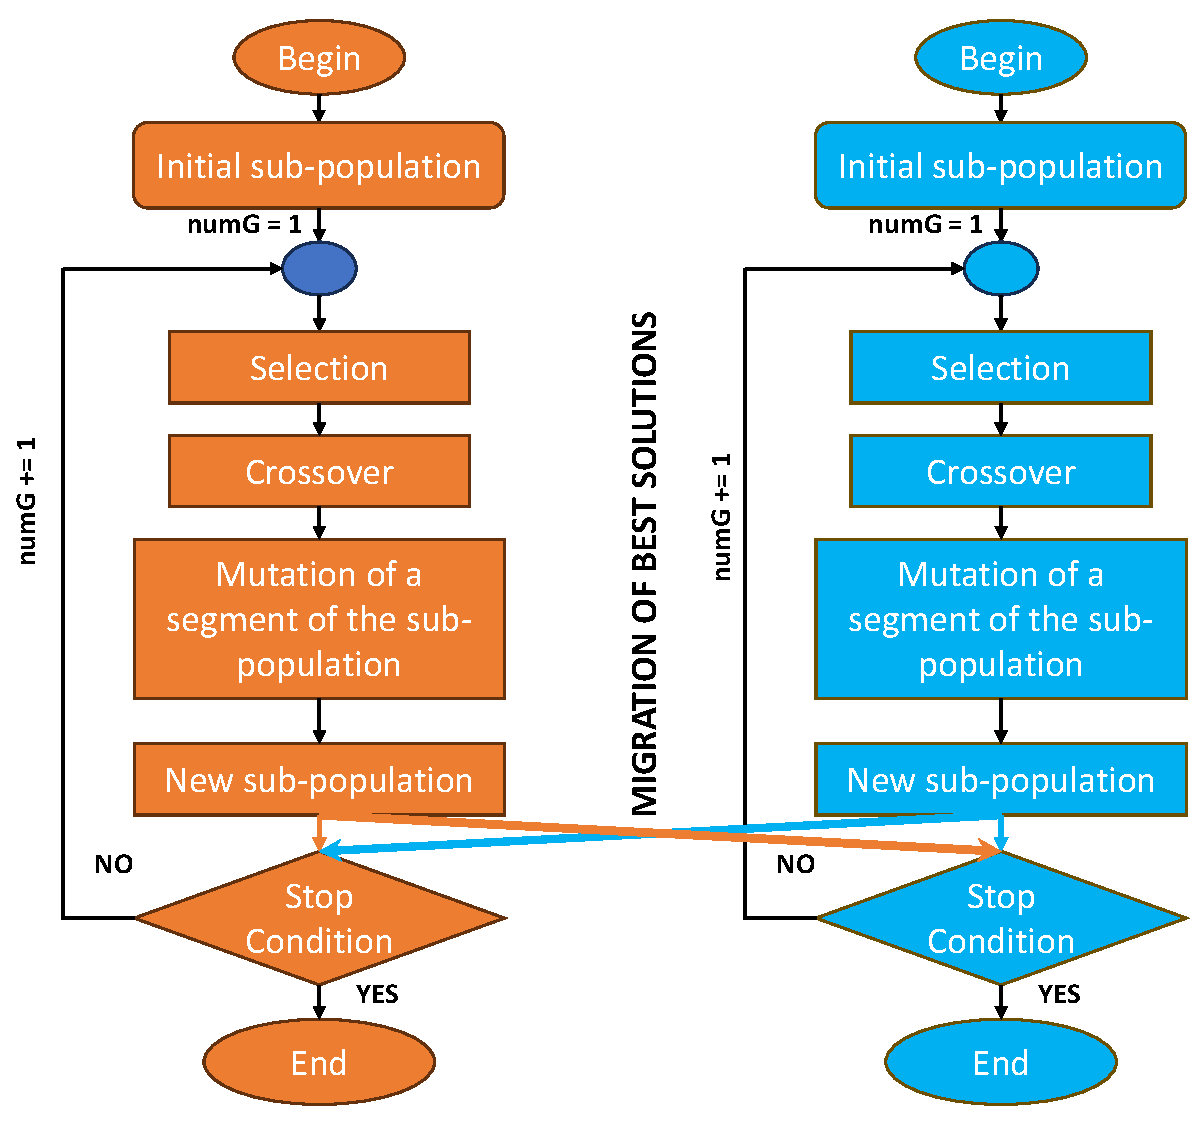
\includegraphics[scale=0.6]{figurePaper/parallelGA.pdf} 
		\caption{\label{Fig1: Figure 1} General Schema of a parallel Genetic Algorithm}
	\end{figure}
\end{center}

\section{Encoding schemes}
In genetic algorithms (GAs), the encoding scheme plays a crucial role in representing candidate solutions to the optimization problem at hand. The choice of encoding directly impacts the performances of the GA, and ultimately, the quality of solutions produced. In this section, we explore the two encoding schemes employed by the sub-populations.

\subsection{Direct Vertex Assignment Encoding (DAVE)}

This representation was first used by \cite{venugopal_narendran_1992} for solving the machine cell formation problem and has been used later on by the majority of papers that adopt an evolutionary approach. The solutions are represented through a vector of length |V| (representing the number of vertices in the graph), wherein each allele denotes the cluster hosting the corresponding vertex, as illustrated in Figure \ref{Fig1: Figure 1}. In which, both $v_1$ and $v_2$ are assigned to the first cluster, which explain the fact that share the same value within the chromosome. 

\begin{center}
\begin{figure}[H]
	\centering
	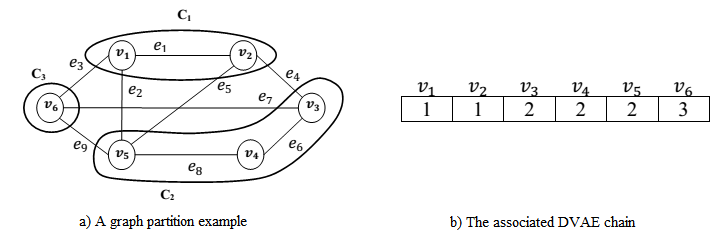
\includegraphics[scale=0.6]{figurePaper/figure1.png} 
	\caption{\label{Fig1: Figure 1} A graph partition example with three clusters and its representative DVAE chain}
\end{figure}
\end{center}

\subsection{Binary string representation }
Introduced by Boulif [2006] and Armbruster et al [2006], to resolve the machine cell formation problem, this encoding scheme uses a vector (chromosome) of length $|E|$ to represent candidates solutions. The value of each allele of the chromosome is either $0$ or $1$. Zero alleles correspond to \textbf{intra}-cluster edge (vertices forming the extremities of this edge are in the same cluster) and ones allele represent (generally) the edge cut or \textbf{inter}-cluster edge vertices forming the extremities of this edge are in two different clusters). Figure \ref{Fig1: Figure 2} blow gives more details.

\begin{figure}[H]
	\begin{minipage}{.5\textwidth}
		\centering
		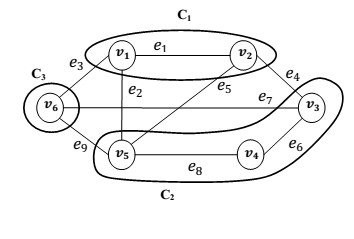
\includegraphics[scale=0.6]{figurePaper/figure2.png}
		%\captionof {}{a) A graph partition example}
		\label{fig}
	\end{minipage}
	\begin{minipage}{.5\textwidth}\centering
		\begin{tabular}{|c|c|c|c|c|c|c|c|c|}
			\hline
			1 & 0 & 1 & 0 & 1 & 1 & 1 & 1 & 0 \\
			\hline
		\end{tabular}	
		%\captionof{}{b) The associated representative chain }
	\end{minipage}
	\begin{center}a) A graph partition example \hspace*{1.cm}   b) The associated representative chain \end{center}
	\caption{A graph partition example with three clusters and its representative binary string encoding.}
	\label{codageBinaire}
\end{figure}

The partition is gotten by recovering the connected components formed by the intra-cluster edges. For the figure bellow, the cluster $C_1={v_1,v_2}$ formed by the intra-cluster edge $e_1$, the second cluster $C_2={v_3,v_4}$ formed by the intra-cluster edge $e_6$, the remaining vertex $v_6$ form the last cluster $C_3$.\\

\noindent \textbf{Remark 1:} The authors assume that the graph is connected. If it is not, they connect it by adding fictive edges with null weights \cite{boulif_atif_2006}.


\section{Experimental Study}
This section is dedicated for the description of the data used in our study, settling of the different parameters along with the metrics employed to measure the performance of the pGA, and at the end presenting and discussing the obtained results according to the chosen metrics.
\subsection{Data description}
For our experimental study we have selected a set of twenty graphs from the literature [Ali and Boulif 2018], the table below illustrates the characteristics of this dataset.
\begin{landscape}
\renewcommand{\arraystretch}{1}
\begin{center}
\begin{table}[H]
\tiny
\begin{tabular}{ccc cc cc c c c c}
\hline
 & \multirow{3}{*}{Reference} & \multirow{3}{*}{Code} & \multirow{3}{*}{$|V|$} & \multirow{3}{*}{$|E|$}  &  \multirow{3}{*}{Density}  & \multirow{3}{*}{Total flow}  & \multicolumn{3}{c}{Constraints} \\
\cline{8-10}
Graph  & • & • & • & • & • & • & Max          & Cohabitation & Non  \\
Number & • & • & • & • & • & • & cluster size &    &cohabitation\\
\hline 
1	& \citep{dimacs10}	& DEBR4	 & 8 &  10  & 0.36 					& 10    &  4  &  (1,4)  (3,6) &         -														\\
2	& \citep{merchichi2015constraint}	& C13  & 10 &  15  & 0.33 	& 15    &  5  & - &    (2,3)  													\\
3	& \citep{merchichi2015constraint} & C8 & 12 &  22  & 0.33 		& 102   &  4  &  (3,6)  (7,8) &  (1,10) 												\\
4	& \citep{dimacs10}	& cage\_3\_5  & 14 &  21  & 0.23 			&  21   &  5  &  (1,2) &  -  																\\
5	& \citep{merchichi2015constraint}& C10	 & 15 &  55 & 0.52 		& 184   &  5  &  (5,14) & (7,10) (14,4)												\\
6	& \citep{dimacs10}	& BFLY & 24 &  36  & 0.13 					& 36    &  8  &  (5,6) & (14,16) 																	\\
7	& \citep{chrisWalshaw}	& Myciel4 & 30 &  45  & 0.10 			& 45    &  6  &  (5,7) & (8,10) 									 						\\

8	& \citep{chrisWalshaw}	& Queen7\_7  & 36 &  290  & 0.46 		& 290   &  12  &  (10,15) &   (3,6) (5,9) 												\\
9	& \citep{chrisWalshaw}	& Queen8\_8	 & 49 &  476  & 0.40 		& 476   &  16  &  (5,6)  (8,11) & (2,3) 												\\
10	& \citep{chrisWalshaw}	& Queen6\_6	 & 74 &  301  & 0.11 		& 301   &  12  &  (4,6)  (5,9) & (23,31) 												\\
11	& \citep{chrisWalshaw}	& Queen8\_12 & 96 &  1368  & 0.30 		&  1368 &  16  &  (35,42) & (1,3)(7,9) 												\\
12	& \citep{chrisWalshaw}	& Queen10\_10 & 100 &  1470  & 0.30 	& 1470  &  20  &  (52,64)  (58,78) &        (16,68) (85,92) 						\\
\hline                                                              
13	& \citep{chrisWalshaw}	& Queen11\_11 & 121 &  1980  & 0.27 	& 1980  &  16  &  (13,15)  (45,46) &        (7,89)   (8,99)   (10,120) 				 \\
14	& \citep{dimacs10}	& SE7 & 128 &  190  & 0.02 					& 190   &  25  &  (15,17)  (24,25)  (42,45)  (56,58) &       (18,43)   (25,40)   (15,96) 		\\
15	& \citep{chrisWalshaw}	& Queen12\_12 & 144 &  2596  & 0.25 	& 2596  &  30  &  (16,23)  (44,56)  (79,85) &       (13,26) 						\\
16	& \citep{dimacs10}	& Bcsstk05 & 153 &  1135  & 0.10 			& 1135  &  50  &  (18,22)  (25,32)  (95,103) &      (15,89)   (24,35)   (42,102) 			\\
17	& \citep{chrisWalshaw}	& Queen13\_13 & 169 &  3328  & 0.23 	& 3328  &  30  &  (4,6)  (5,9)(52,64)(58,78) &(10,21)(15,19)(16,25)   (18,32) 		\\
18	& \citep{chrisWalshaw}	& Queen14\_14 & 196 &  4147  & 0.22 	& 4147  &  35  &  (121,125)  (132,145)  (156,160) &(4,6)(5,9)(52,64)(58,78) 		\\
19	& \citep{chrisWalshaw}	& Queen15\_15 & 225 &  5180  & 0.21 	& 5180  &  40  &(25,62)(143,156)(174,182)&(121,125)(132,145)(156,160) 				\\
20	& \citep{dimacs10}	& G250.04 & 250 &  613  & 0.02 				& 613   &  30  &  (2,3)  (113,153)  (150,210)  (240,243) &   (143,182)   (213,245) 			\\
\hline
\end{tabular} 
\caption{\label{GraphInstances} Graph instances}
\end{table}
\end{center}
%----------------------------------------------------------------------------------------------------------------------------------------------------------------
\end{landscape}


 

\subsection{pGA parameters}
Table 1 summarize the set of pGA parameters and their respective values. It is worth to mention that these values are settled empirically through a set of experiences.

\begin{table}[H]
	\center
	\label{tab:AG} % pour les référence croisées
	\begin{tabular}{c c}
		\hline
	    \bf  Parameters & Values \\
		\hline 
			 Sub-population size  & 100 \\
			 Elitism rate   & 10 \\		 
			 Reproduction rate   & 10 \\
			 Mutation rate   & 0.02 \\
			 Number of runs   & 10 \\	
			 Number of iterations   & 100 \\	
			 Migration frequency   & 10 \\	   		 		
		\hline
	\end{tabular}
\end{table}

\subsection{pGA Metrics }
In order to compare the performances of the GA using explained encoding schemes, we use three metrics; two of them are used to compare the efficiencies of the representations namely \textbf{ART} (Average Run Time) which is the average of the run time obtained over the thirty runs corresponding to the best solution of each run and \textbf{AES} (Average Evaluation to a Solution) is the average number of solutions visited in the search space by the GA to get the best one all over the runs. In the other side, the \textbf{ABF} (Average Best Fitness) which is the average of the best fitness obtained by the runs, is used to compare effectiveness (solution quality) of the GA using the representation methods. [Eiben 2011].
The material used to achieve our experiences consist of a PC with an Intel(R) Core(TM) i5-4200U 2.6 HZ and a RAM of 6 Go. 
\section {Discussion of the Experimental Results}
We next report our findings. As expected, combining different encoding schemes using a parallel genetic algorithm leads to better results and enhance the performances of the GA. The following graphics illustrates clearly the outclassing of the pGA over the GAs each of them using a unique encoding scheme either in terms of the MBF and BF metrics. Indeed Figure \ref{MBF_METRIC}, depicts the superiority of the pGA against the other GAs in terms of MBF. Furthermore, for some instance where the GAs failed to reach at least a feasible solution that fulfilled all the constraints, the pGA provide a good score.
\begin{center}
	\begin{figure}[H]
		%\centering
		\begin{subfigure}{0.45\textwidth}
			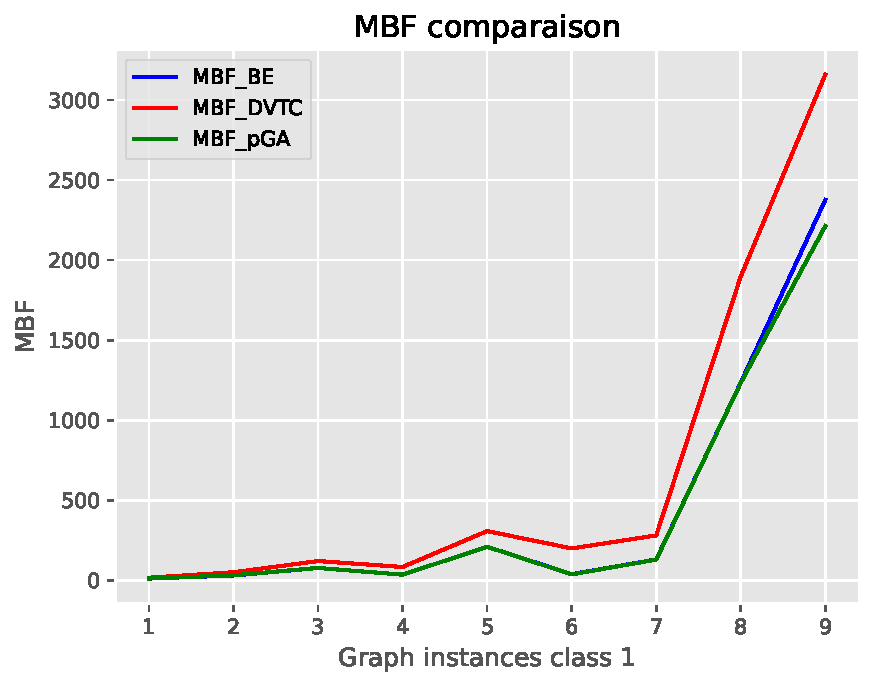
\includegraphics[width=\textwidth]{figurePaper/MBF_C1.pdf} 
			\caption{\label{MBF_METRIC_C1} graph instances class 1 from 1 to 10}
		\end{subfigure}
		\hfill
		\begin{subfigure}{0.45\textwidth}
			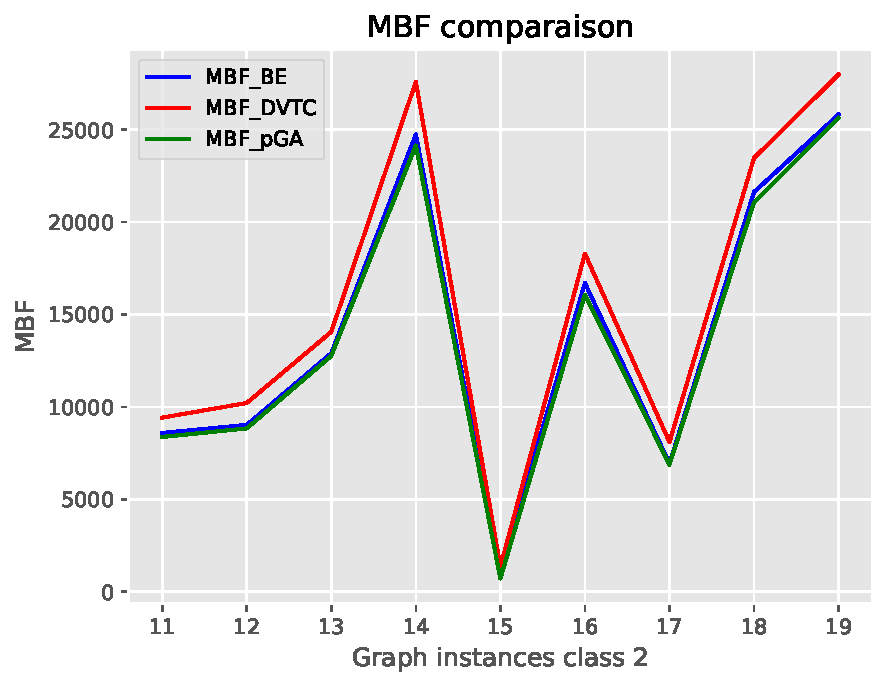
\includegraphics[width=\textwidth]{figurePaper/MBF_C2.pdf} 
			\caption{\label{MBF_METRIC_C2} graph instances class 1 from 11 to 20}
		\end{subfigure}
		\caption{\label{MBF_METRIC}pGA performances according to MBF metric}
		
	\end{figure}
\end{center}
Considering the ART metric, the pGA scores are compared to the worst scores of the GAs. Nonetheless, knowing that the pGA is combining all the GAs, it is obvious that its run time is compared to the GA giving the worst score in terms of ART which the BE encoding. Figure \ref{ART_METRIC} shows the graphic comparing the methods in terms of ART metric.
\begin{center}
	\begin{figure}[H]
		%\centering
		\begin{subfigure}{0.45\textwidth}
			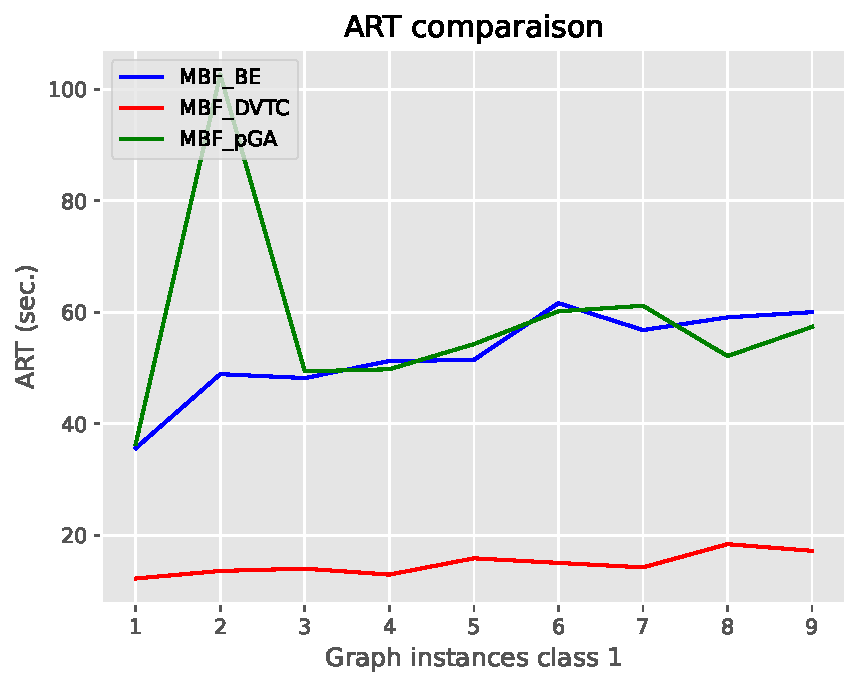
\includegraphics[width=\textwidth]{figurePaper/ART_C1.pdf} 
			\caption{\label{ART_METRIC_C1} graph instances class 1 from 1 to 10}
		\end{subfigure}
		\hfill
		\begin{subfigure}{0.45\textwidth}
			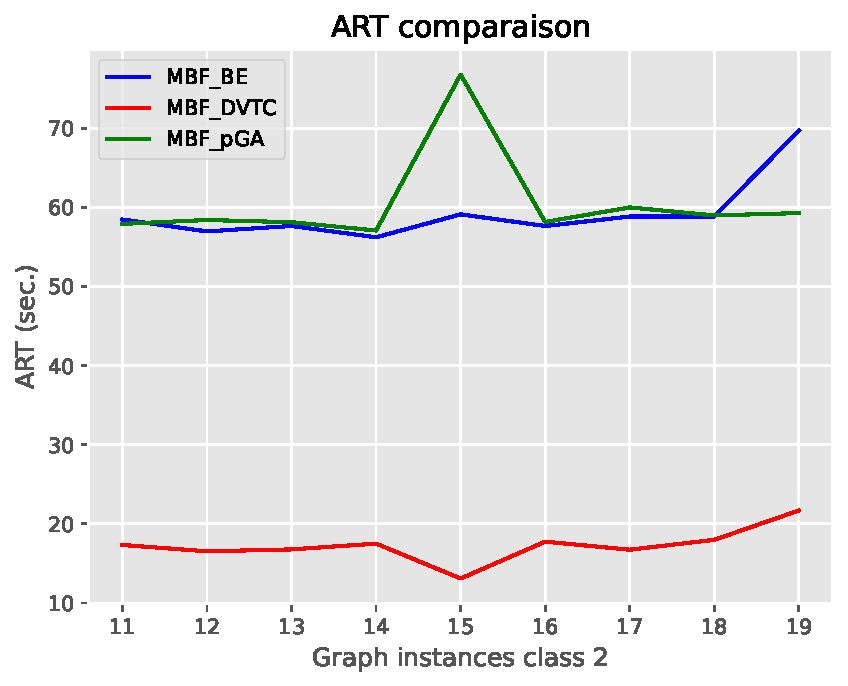
\includegraphics[width=\textwidth]{figurePaper/ART_C2.pdf} 
			\caption{\label{ART_METRIC_C2} graph instances class 1 from 11 to 20}
		\end{subfigure}
		\caption{\label{ART_METRIC}pGA performances according to ART metric}
		
	\end{figure}
\end{center}
When coming to the AES metric,  pGA gets the worst scores, however taken with the MBF and BF metrics, this will highlights a crucial point in favor of the pGA. In fact, having a height AES with a good MBF means that the pGA had deeply explore the search landscape and get through an important number of solutions to bring at the end the best one it could reach.
\begin{center}
	\begin{figure}[H]
		%\centering
		\begin{subfigure}{0.45\textwidth}
			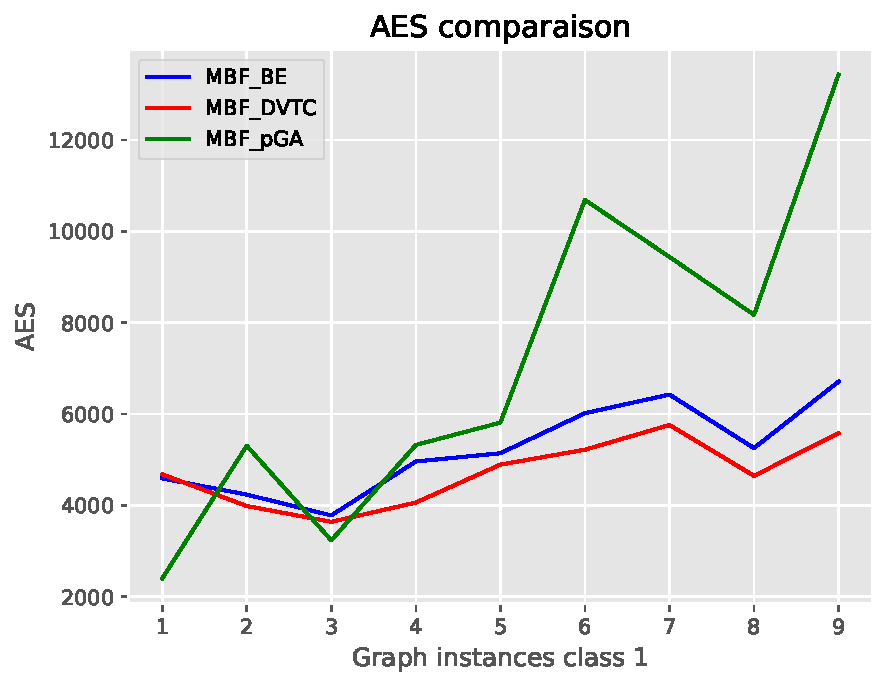
\includegraphics[width=\textwidth]{figurePaper/AES_C1.pdf} 
			\caption{\label{AES_METRIC_C1} graph instances class 1 from 1 to 10}
		\end{subfigure}
		\hfill
		\begin{subfigure}{0.45\textwidth}
			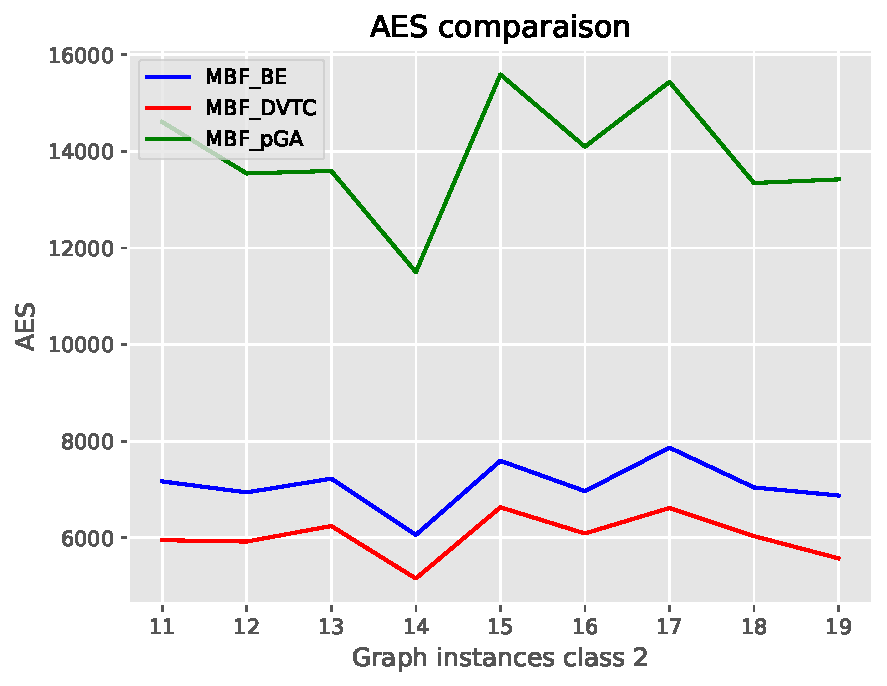
\includegraphics[width=\textwidth]{figurePaper/AES_C2.pdf} 
			\caption{\label{AES_METRIC_C2} graph instances class 1 from 11 to 20}
		\end{subfigure}
		\caption{\label{AES_METRIC}pGA performances according to AES metric}
		
	\end{figure}
\end{center}
Indeed, simultaneously evolving multiple sub-populations through a parallel Genetic Algorithm (pGA) with a suitable migration strategy serves as a valuable tool in steering the search process of a specific encoding scheme towards alternative regions that hold potential for achieving superior solutions. This collaborative approach assists encoding schemes in surpassing their inherent limitations.

\section{Conclusion}
In conclusion, the utilization of a parallel genetic algorithm employing diverse encoding schemes for its sub-populations presents a promising approach in addressing the graph partitioning problem. Through our investigation, it becomes evident that the pGA outperforms the traditional GA. By harnessing the collaborative power of multiple encoding schemes and leveraging effective migration strategies, the pGA demonstrates its capability to overcome the inherent challenges of the graph partitioning problem. As perspective to this work, we plan to use more than two sub-population with a more elaborated migration strategy to elevate the performances of the pGA.






\section*{References}
\bibliography{referencesBib.bib}
\end{document}
